\documentclass{article}
\usepackage[utf8]{inputenc}
\usepackage[spanish]{babel}
\title{Modelos matemáticos discretos}
\author{bl}
\begin{document}
\maketitle
\section{Ecuaciones en diferencias}
\subsection{Primer orden}

Sabemos que $$\lim_{x\to\infty}\frac{1}{x}=0$$.

Tenemos \$1000 que vamos a invertir en un interés de 1\% mensual. 

El valor de la inversión cuando han transcurrido $n$ meses es $$x_n=1000(1.01)^n$$

\begin{center}
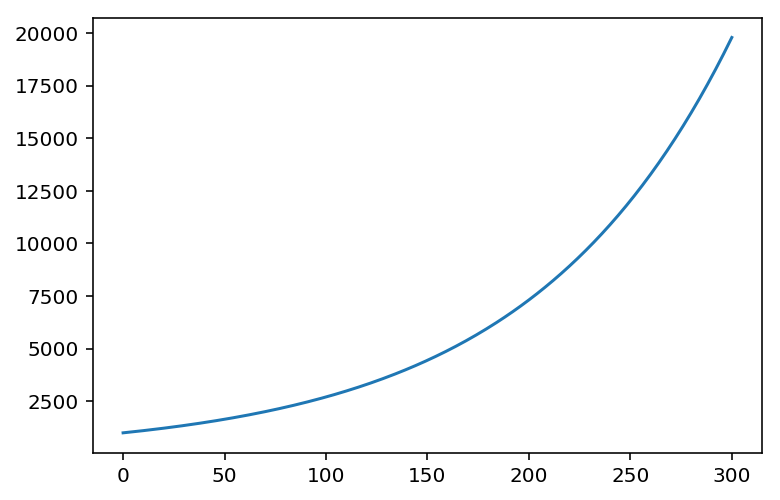
\includegraphics[width=8cm]{grafica}
\end{center}

\subsection{Segundo orden} 

\end{document} 
